\chapter{\label{chap:lit-review}Revisão Bibliográfica}

\section{Spelunky}
Spelunky \cite{SPELUNKYWEB} é um jogo onde o jogador incorpora um aventureiro
que decide explorar uma caverna misteriosa. O local contém tesouros, mas também
está repleto de perigos. O objetivo principal do jogador é explorar estas
cavernas subterrâneas e coletar a maior quantia de tesouros possível enquanto
evita ser abatido pelos diversos inimigos e armadilhas espalhadas pelo ambiente.
O jogo 2D segue o estilo \textit{platformer} - tipo de jogo que envolve guiar um
personagem através de plataformas suspensas e obstáculos para obter progresso no
jogo.

O jogo faz uso de alguns dos elementos-chave do gênero \textit{roguelike} --
gênero de jogos que se tornou popular nos anos 80 caracterizado por sua
dificuldade extrema, enfoque em exploração de ambientes e narrativa fantasiosa
--, como \textbf{geração procedural} e \textbf{morte permanente}. Os níveis em
Spelunky são gerados proceduralmente - ou seja, utiliza um algoritmo capaz de
gerar automáticamente os elementos que irão compor o nível - fazendo com que
cada partida seja única. Isto significa que não existe uma maneira de se
memorizar estratégias específicas de um mapa em Spelunky, pois ao início de cada
partida o mapa é gerado de maneira única e os tesouros, itens e obstáculos são
dispostos de maneira diferente, fazendo com que o jogador tenha que aprender a
lidar com os elementos de forma individual, combinar este conhecimento e
estabelecer uma estratégia para vencer seus obstáculos e ser bem sucedido. Além
disso, o jogo conta com o conceito de morte permanente, que faz com que o
jogador, ao ter o seus pontos de vida esgotados, tenha que recomeçar o jogo
desde o seu início, perdendo todo o progresso obtido até então.

O jogo é dividido em 4 áreas principais: \textbf{As Minas}, \textbf{A Selva},
\textbf{As Cavernas De Gelo} e \textbf{O Templo}. Cada área possui um estilo de
mapa e aparência única. O nível de dificuldade também aumenta gradativamente
conforme o jogador avança pelas áreas, principalmente porque os inimigos
vão se tornando cada vez mais fortes. Além das áreas principais, existem duas
áreas secretas: \textbf{O Mercado Negro} e \textbf{A Cidade de Ouro}.

O jogador, inicialmente, conta somente com um chicote, 4 pontos de vida, 4
bombas e 4 cordas. Contudo, pode obter e utilizar diversos equipamentos,
acessórios e armas ao longo do jogo. Além disso, o jogador pode interagir com
objetos do ambiente, como pedras, vasos, baús de tesouro, entre outros. Também
se encontram, espalhados pelas cavernas, os \textbf{Comerciantes}. Estes
\textit{NPCs}\footnote{\textit{Non-Playable Characters} (Personagens Não-
Jogáveis). São personagens que não são controlados pelo jogador. Geralmente
interagem de alguma maneira com o personagem do jogador.} comercializam itens
com o jogador em troca de tesouros. É possível, inclusive, tentar furtar itens
destes comerciantes. Contudo, se o jogador o fizer, todos os comerciantes
ficarão extremamente irritados e passarão a caçar o explorador com espingardas.

O jogo foi desenvolvido por Derek Yu - utilizando o motor de desenvolvimento de
jogos \textit{GameMaker} (Versão 8.0 Pro) - e lançado gratuitamente para a
plataforma \textit{Windows} em dezembro de 2008 \cite{SPELUNKYRELEASE}. No fim
de 2009, o criador optou por liberar o código fonte do jogo, permitindo sua
distribuição não-comercial e modificação \cite{SPELUNKYLICENSE}. A liberação do
código fonte de Spelunky pode ser considerada um marco muito importante, pois
permitiu que fossem criadas modificações para o jogo. Estas modificações, que
podem ser encontradas no fórum oficial da
\textit{Mossmouth}\footnote{Disponível em:
http://mossmouth.com/forums/index.php} -- empresa desenvolvedora de jogos
criada por Derek Yu --, são correções de \textit{bugs}, mapas customizados ou
até mesmo modos de jogo completamente diferentes do jogo original. Pode-se
dizer que dar esta liberdade para a comunidade do jogo é um dos fatores que
ajuda a manter sua base de jogadores e atraem novos jogadores até hoje.

O motor GameMaker disponibiliza diversas ferramentas que facilitam o trabalho
do desenvolvedor. Contando com funcionalidades como editores de
\textit{scripts}\footnote{Código desenvolvido para o controle dos
comportamentos dos elementos do jogo.} e de \textit{sprites}\footnote{Elementos
visuais do jogo, tais como o personagem, o fundo, os inimigos. Representados
como uma ou mais imagens, permitindo que as mesmas sejam animadas.},
gerenciadores de eventos, entre outras \cite{GMAKER8DOCS}, o GameMaker oferece
um ótimo suporte ao desenvolvedor para a criação de jogos. O motor
disponibiliza uma linguagem de programação própria para seus \textit{scripts},
a \textit{GameMaker Language}, ou \textit{GML}.

\begin{figure}[htb!]
\centering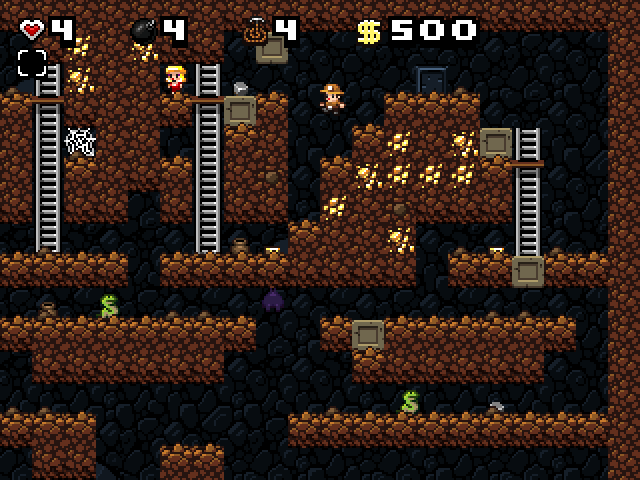
\includegraphics[width=.65\textwidth]{fig/spelunky-pc-screen.png}
\caption {\label{fig:spelunky-gameplay}Exemplo de partida de spelunky, mostrando
elementos do jogo como o jogador, a caverna, os inimigos, os tesouros, entre
outros.} \end{figure}


%----------
\section{Plataformas de Testes para Inteligência Artificial}

Existe uma relação mutuamente benéfica entre a área de inteligência artificial e
jogos digitais.  De um lado, os jogos se beneficiam explorando conceitos,
técnicas e algoritmos de inteligência artificial com o intuito de enriquecer seu
conteúdo. O jogo \textbf{Black \& White}, da desenvolvedora \textit{Lionhead
Studios}, por exemplo, incorporou as técnicas de agentes BDI, árvores de decisão
e redes neurais \footnote{Explicamos o funcionamento destas técnicas na seção
\ref{section:agents}}  para ditar o comportamento de alguns seus personagens
\cite{TOPAIGAMES}.  Já o jogo \textbf{F.E.A.R}, da desenvolvedora
\textit{Monolith Productions}, utilizou os conceitos de planejamento para
aumentar o realismo das decisões tomadas por seus agentes \cite{FEARPLANNING}.
Do outro lado, o campo da inteligência artificial se beneficia ao utilizar os
jogos como plataformas de teste para suas técnicas e algoritmos. Jogos digitais
são atraentes para pesquisadores da área de inteligência artificial porque
capturam a complexidade de situações do mundo real, são relativamente simples e
baratos de desenvolver, podem replicar inúmeras situações e ambientes -- existem
diversos gêneros de jogos, variando desde jogos educacionais até jogos de tiro
em primeira pessoa -- e até mesmo criar cenários impossíveis ou impraticáveis no
mundo real. Ademais, possuem a vantagem de serem programas de computador, o que
significa que, por muitas vezes, podem acelerar a velocidade na qual testes são
executados, ou ainda executar múltiplos testes em paralelo. A natureza lúdica
dos jogos também são um ponto importante a ser ressaltado, pois ajudam a motivar
os pesquisadores, além de resultar na adesão de novos pesquisadores.

Tendo este apanhado de informações em mente, pesquisadores e entusiastas da área
acabam desenvolvendo \textit{frameworks} de inteligência artificial em cima de
jogos existentes para servir de plataforma de teste. Um exemplo disso é o
\textbf{Brood War API} \cite{BWAPI}, um \textit{framework} para o jogo
\textit{StarCraft: Brood War}. Algumas vezes, contudo, são criados jogos
especificamente para isso, como foi o caso do projeto \textbf{TORCS, The Open
Racing Car Simulator}, um simulador de corridas de carro que permite que
desenvolvedores programem a inteligência de carros e compitam entre si
\cite{TORCSWEB}.

\subsection{Competições de Inteligência Artificial em Jogos Digitais}
Muitas vezes, os \textit{frameworks} de inteligência artificial desenvolvidos
abrem espaço para a criação de competições, servindo como base comum para o
desenvolvimento e aplicação de técnicas de inteligência artificial para os
concorrentes. Nestas disputas, os competidores são encorajados a resolver
problemas ou sub-problemas impostos pelo jogo em questão, sendo vencedores os
candidatos que melhor resolvê-los.

Geralmente, o problema proposto é o de jogar o jogo de maneira mais eficiente.
Para realizar uma avalição objetiva, são utilizadas métricas estipuladas pelo
próprio jogo, como pontuação ou tempo. Muitas vezes, os organizadores da
competição optam por fazer uso de um sistema de \textit{ranking}, expondo os
resultados obtidos pelos candidatos. A competição \textbf{The General Video Game
AI Competition}, que explora o problema de criar controladores genéricos de
jogos, faz uso deste mecanismo \cite{GVGAIWEB}.  Às vezes, as competições fazem
com que os candidatos joguem entre sí para avaliá-los.  Um exemplo disso seria a
competição que gira em torno de \textbf{Vindinium}, um jogo para a plataforma
\textit{web} \cite{VINDINIUMWEB}.

Contudo, a proposta principal da disputa pode ser outra. A competição
\textbf{Mario AI Competition}, por exemplo, possuia como uma de suas metas a
criação de níveis interessantes para o jogo \cite{MARIOAIWEB}. Já a competição
\textbf{2K Bot Prize} tinha como objetivo a criação de uma inteligência
artificial para o jogo \textit{Unreal Tournament 2004} que pudesse enganar
outros jogadores e fazê-los pensar que era um humano jogando
\cite{UNREALAIWEB}. Neste tipo de torneio, a avaliação se dá de maneira
subjetiva, visto que não existe uma métrica numérica para determinar diversão,
por exemplo.

Os organizadores destas competições costumam, ao término da disputa,
disponibilizar os códigos-fonte de todos os candidatos. Assim, em versões
futuras da competição, os competidores terão a oportunidade de investigar quais
técnicas e algoritmos foram mais eficientes no passado. Competições onde os
candidatos duelam entre sí tendem a aumentar a competitividade, pois uma
solução que funcionou em um ano pode vir a não funcionar tão bem ou até mesmo
falhar no ano seguinte, tendo em vista que o código será dissecado pelos seus
rivais. Os resultados das competições costumam ser divulgados também em
conferências como \textit{IEEE Computational Intelligence and Games (CIG)} e
\textit{AAAI Artificial Intelligence in Interactive Digital Entertainment
(AAIDE)}, além de conferências dedicadas a computação evolutiva, \textit{game
design}, aprendizado de máquina, entre outras. Algumas competições costumam
oferecer prêmios em dinheiro para os melhores colocados, como forma de
incentivo.


%----------
\section{SpelunkBots}
Utilizando o código-fonte de Spelunky, Daniel Scales e Thomas Thompson, da
Universidade de Derby no Reino Unido, criaram o \textit{SpelunkBots}
\cite{SPELUNKBOTSWEB}, um \textit{framework} que permite a programação de
\textit{bots} para o jogo Spelunky. Um dos objetivos dos criadores é utilizar a
aplicação para criar uma competição de inteligência artificial para o jogo. A
aplicação se comunica com o código-fonte original e permite a utilização das
linguagens \textit{GML} (padrão do GameMaker) e \textit{C++} para a descrição
do comportamento de \textit{bots}.

A \textit{API} possibilita que o desenvolvedor resgate informações de objetos
estáticos e dinâmicos contidos no ambiente do jogo, como o terreno do jogo ou a
posição de tesouros, armadilhas e inimigos. Contudo, o objetivo da \textit{API}
disponibilizada por SpelunkBots é fazer com que a informação recebida pelo
\textit{bot} se assemelhe ao máximo com a percepção de um jogador humano.  Para
tal, o \textit{framework} implementa um sistema de \textit{fog of war},
limitando o conhecimento do ambiente que pode ser obtido pela inteligência
artificial.  Para objetos estáticos, uma vez que o jogador visualizou o objeto
ele poderá receber informações sobre ele permanentemente. Para objetos
dinâmicos, o \textit{bot} só poderá receber informações sobre eles se os mesmos
estiverem sendo visualizados por ele. A imagem \ref{fig:spelunkbots-fow} ilustra
um exemplo de funcionamento do sistema.

\begin{figure}[htb!]
\centering
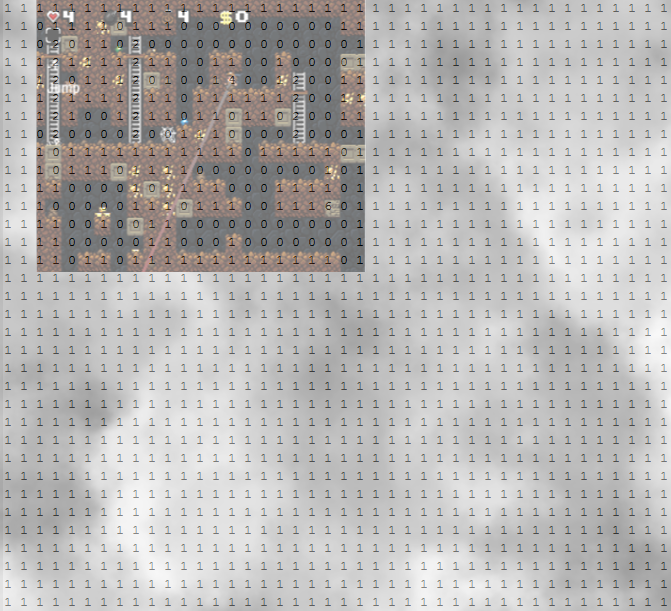
\includegraphics[width=.65\textwidth]{fig/spelunkbots-fow.png}
\caption {\label{fig:spelunkbots-fow}Visualização do sistema de textit{fog of
war} demonstrando a diferença de informação recebida de elementos dentro e fora
do campo de visão do jogador.}
\end{figure}

Para permitir que o \textit{bot} execute ações, o desenvolvedor pode enviar
comandos através da simulação de aperto de botões. Os comandos são enviados após
o processamento realizado pelo \textit{bot}, ao fim de cada atualização do jogo.
O resultado das ações executadas depende de quais itens o jogador tem equipado
no momento. Por exemplo, enviar um comando de salto enquanto o jogador possui um
\textit{jetpack} equipado fará com que ele salte mais alto. Tendo isto em mente,
a \textit{API} permite que o desenvolvedor saiba quais itens o jogador possui
atualmente.

O jogo original foi modificado para possibilitar que o jogador crie níveis
customizados e pule para qualquer nível ou área do jogo, caso queira testar as
capacidades de seu \textit{bot} em cenários específicos ou mais difíceis sem ter
que jogar o jogo desde o início. O SpelunkBots também conta com uma opção de
acelerar ou desacelerar a partida. Isto facilitaria a implementação de uma
abordagem focada em aprendizado de máquina, pois aceleraria o processo de
aprendizado. O \textit{framework} oferece ao desenvolvedor a capacidade de
visualizar informações importantes -- como, por exemplo, o estado do
\textit{bot}, sua trajetória e o ambiente -- diretamente na tela do jogo,
enquanto o programa está em execução. Os criadores da competição disponibilizam
alguns \textit{bots} e níveis básicos para exemplificar a utilização da
\textit{API}, fornecendo, assim, uma base inicial aos competidores.

\begin{figure}[htb!]
\centering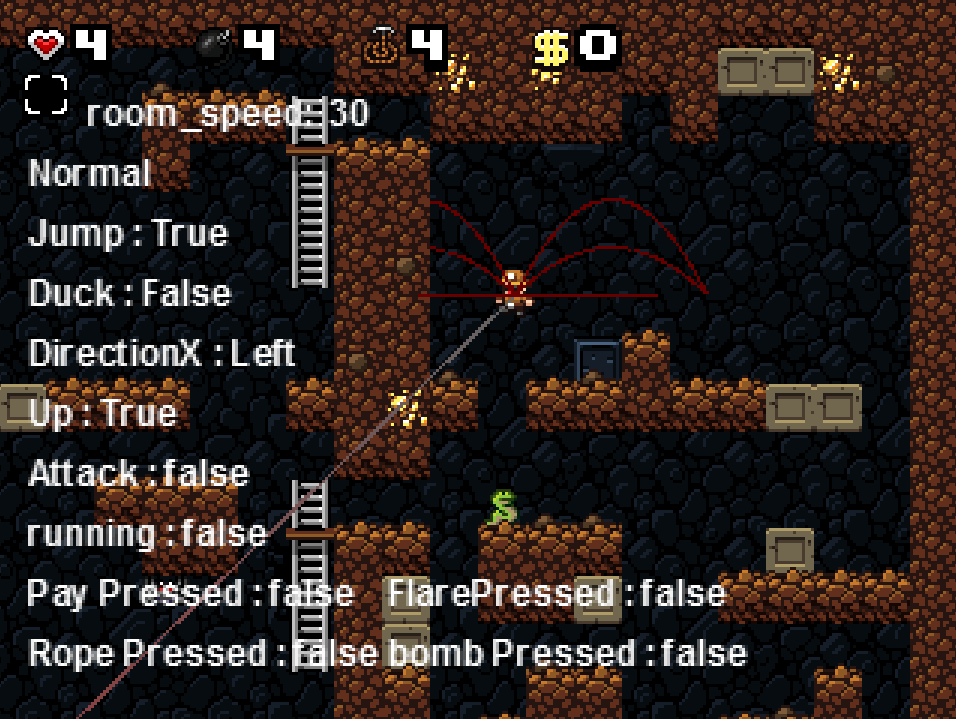
\includegraphics[width=.65\textwidth]{fig/spelunkbots-debug-screen.png}
\caption {\label{fig:spelunkbots-debug-screen}Tela capturada para demonstrar
algumas das informações de \textit{debug} disponíveis durante a execução do
programa SpelunkBots.} \end{figure}


%----------
\section{\label{section:agents}Agentes Racionais}
Um agente pode ser visto como uma entidade capaz de utilizar seus sensores para
perceber o ambiente onde está situado, atuando nesse ambiente conforme sua
necessidade através de elementos atuadores \cite{Russell:1995:AIM:193191}.
Para exemplificar, podemos tomar como exemplo o ser humano, que consegue
perceber o ambiente através de seus sentidos -- tais como visão e audição --,
atuando neste com suas partes do corpo, como braços, pernas, mãos, etc
\cite{Russell:1995:AIM:193191}.  Portanto, podemos generalizar o conceito de
agente racional como todo e qualquer tipo de agente que, no ambiente em que
está inserido, toma ações que o deixam mais próximo de completar os objetivos
os quais o mesmo está comprometido.

\textbf{Agentes reflexivos} são agentes que executam ações baseados em alguma
situação percebida. Por exemplo, podemos ter um agente reflexivo que poderá
fazer uma postagem em uma rede social, dado que uma outra pessoa fez uma
postagem. Este tipo de agente simplesmente executa uma ação baseado no que
percebeu anteriormente. Tais agentes têm como principal característica não
guardarem tipo algum de informação das suas experiências passadas, sendo apenas
reativos.

Diferentemente dos agentes reflexivos, \textbf{agentes com memória} são capazes
de guardar informações sobre as experiências passadas, podendo fazer o uso das
mesmas para alcançar seus objetivos. A lembrança das experiências passadas
fornece ao agente uma oportunidade de utilizar melhor os seus recursos, sendo
capaz de investí-los em ações mais efetivas do que as tomadas em experiências
passadas.

Além de ter memória, é necessário que um agente saiba quando obteve sucesso no
que se propôs a fazer. Com isso, \textbf{agentes baseados em objetivos}
conseguem tomar suas decisões com base na ação que os deixa mais próximos de
alcançarem seus objetivos. O desafio desse tipo de agente é saber como alcançar
esse objetivo, podendo ser usadas técnicas de busca e planejamento para
determinar as possíveis ações a serem executadas para alcançá-lo.

Para alguns tipos de agente, chegar no objetivo pode não ser suficiente,
podendo existir outros fatores na busca desse objetivo que possam influenciar
no resultado final para agente. Por exemplo, um agente que joga um determinado
jogo pode finalizar a partida com um certo número de pontos, porém, é mais
satisfatório que termine o jogo com o \textbf{maior} número de pontos
possível. Estes são os \textbf{agentes baseados em utilidade}, que, de um
conjunto de ações disponíveis, selecionam e executam a que seja mais vantajosa.

\subsection{Ambiente}
Todas as ações que um agente pode executar, bem como suas percepções, ocorrem
no \textbf{ambiente} onde o agente está inserido. Porém, existem diferentes
tipos de ambientes, que, dependendo de sua dimensão, podem dificultar o trabalho
de um agente. Podemos classificar os ambientes em \textbf{acessíveis} ou
\textbf{inacessíveis} (também chamados de \textbf{observáveis} ou \textbf{não
observáveis}), \textbf{determinísticos} ou \textbf{estocásticos},
\textbf{episódicos} ou \textbf{sequenciais}, \textbf{dinâmicos},
\textbf{semi-dinâmicos} ou \textbf{estáticos} e \textbf{discretos} ou
\textbf{contínuos}.

Um ambiente é \textbf{acessível} caso seja possível perceber os estados do
ambiente através dos sensores de um agente, sendo \textbf{inacessível} caso
contrário. Quando um agente tem certeza do próximo estado ao executar uma ação
no ambiente, trata-se de um ambiente \textbf{determinístico}, quando não se tem
essa certeza, chamamos o ambiente de \textbf{estocástico}. Também existem
ambientes \textbf{episódicos} ou \textbf{sequenciais}, sendo ambientes
episódicos aqueles onde um episódio não influencia no próximo. Dessa forma,
ambientes sequenciais guardam algum tipo de memória dos episódios anteriories,
usando essa memória nos episódios subsequentes, gravando outras informações
sobre estes caso necessário. Caso um ambiente possa sofrer mudanças sem ações
do agente, será um ambiente \textbf{dinâmico}. Caso contrário, chamamos esse
tipo de ambiente de \textbf{estático}. Se o ambiente não muda de acordo com o
tempo, mas o agente muda sua maneira de agir (melhorando sua atuação, por
exemplo), chamamos o ambiente de \textbf{semi-dinâmico}. Por fim, classificamos
os ambientes como \textbf{discretos} ou \textbf{contínuos}, sendo ambientes
discretos aqueles onde se têm um número finito de ações possíveis e de
percepções.

\subsection{Agentes BDI}
O estudo de agentes racionais faz com que seja necessário, além de
compreender seus aspectos e características, entender como é possível
realizar a implementação desse tipo de agente. A aplicação de técnicas
convencionais para o desenvolvimento desses agentes é despendiosa e
difícil de ser feita, verificada e mantida \cite{bdi-icmas95}, sendo
então necessário o uso de outras técnicas para sua implementação.

Nesse contexto, surge a arquitetura de agentes BDI (sigla para \textit{Belief,
Desire, Intentions}), capaz de modelar agentes racionais de uma maneira mais
adequada. Tal arquitetura conta com alguns conceitos que permitem modelar
agentes racionais, explicados a seguir:

\begin{description}
\item [Crenças (\textit{Beliefs})]
Tudo aquilo que o agente acredita saber sobre o ambiente é chamado de
``crença'', pois tal informação pode vir a não ser verdade.  As crenças são
atualizadas e armazenadas na memória do agente a cada nova percepção do
ambiente feita por ele.

\item [Desejos (\textit{Desires})]
Além de uma base de crenças, é necessário que um agente saiba o que deve ser
feito para alcançar os seus objetivos. Tais ações são chamadas de desejos e
representam o que um agente deseja fazer, além de descreverem os custos
associados com a busca por este desejo.

\item [Intenções (\textit{Intentions})]
Diferentemente dos desejos, uma intenção é algo com o qual o agente se
compromete a fazer em busca dos seus objetivos. Dessa forma, podemos ver as
intenções como as ações que efetivamente serão executadas para alcançar os
objetivos.
\end{description}

Com estes três conceitos, é possível definir um algoritmo interpretador de
agente BDI. O algoritmo~\ref{alg:BDIINTERPRETERALG} mostra como é feito o uso
desses conceitos \cite{BDIFROMTHEORYTOPRACTICE}.

\begin{algorithm}[htb] \begin{center}
	% Um exemplo de algoritmo utilizando a pacote 'algorithmic'
	%\algsetup{linenosize=\small,linenodelimiter=.}
	\begin{algorithmic}[1] \STATE inicializar(); \STATE \WHILE {true} \STATE
	opções $\gets$ gerar-opções(fila-de-eventos); \STATE opções-escolhidas
	$\gets$ deliberar(opções); \STATE atualizar-intenções(opções-escolhidas);
	\STATE executar(); \STATE buscar-novos-eventos-externos(); \STATE
	esquecer-atitutes-de-sucesso(); \STATE esquecer-atitudes-impossíveis();
	\ENDWHILE \end{algorithmic} \end{center} \caption[Algoritmo para representar
	um interpretador de agente BDI.] {\label{alg:BDIINTERPRETERALG} Algoritmo
	para representar um interpretador de agente BDI, utilizando os conceitos de
	crenças, desejos e intenções para a sua implementação.} \end{algorithm}

As possíveis opções são escolhidas a cada novo ciclo, sendo sempre buscadas de
uma fila de eventos ocorridos. Após, é escolhida uma opção a ser seguida,
tornando-se então essa opção uma intenção do agente. Caso haja uma intenção a
ser executada, o agente então a executa. A seguir, é atualizada a fila de
eventos com os eventos externos ocorridos. Por fim, o agente esquece os desejos
já obtidos, as intenções satisfeitas e os desejos e intenções impossíveis.

Cabe ressaltar que tal arquitetura possui algumas limitações, como a
incapacidade de fazer com que um agente BDI ``aprenda'' e adapte seu
comportamento baseado no conhecimento obtido, além de não haver nenhuma
consideração arquitetural sobre a modelagem de sistemas multi-agentes
\cite{Georgeff:1998:BMA:648205.749450}, sendo assim necessário explorar
outras técnicas caso seja necessário que o agente faça uso dessas
características.

\section{Planejamento}

A solução para muitos tipos de problemas pode ser expressa através de uma
sequência de ações a serem executadas -- isto é, um plano --, principalmente
quando temos algum tipo de restrição no ambiente. Portanto, em muitos casos, é
necessário que um agente estabeleça um plano de ações para resolver o problema
ao qual foi designado a solucionar.

Tomemos como exemplo um agente em um ambiente estocástico -- onde não se
consegue ter certeza sobre o resultado da execução de uma ação -- e
não-observável. Como não temos certeza sobre o estado do ambiente, nem sobre o
resultado de nossas ações, precisamos estabelecer um plano onde podemos tratar
as dificuldades que o ambiente nos impõe.

Portanto, podemos definir um sistema planejador como um sistema que tem como
saída um plano a ser executado e como entrada os seguintes componentes
\cite{Woolridge:2001:IMS:559667}:

\begin{description}
\item [Objetivos]
Também chamados de intenções ou tarefas. É algo que o agente deseja obter,
manter ou evitar.

\item [Crenças]
Tudo o que um agente sabe sobre o estado do ambiente.

\item [Ações]
Tudo o que um agente pode executar no ambiente onde está inserido.
\end{description}

A ideia principal para a construção de um sistema planejador se dá através da
extensão da representação de crenças, objetivos e ações com o uso de algum tipo
de linguagem formal (normalmente lógica de primeira ordem, ou algum subconjunto
da mesma). Isso permite que o planejador possa fazer uma ligação direta entre as
ações e os estados, podendo, portanto, considerar apenas ações relevantes para o
plano \cite{Russell:1995:AIM:193191}. As ações passam a ter pré-condições e
efeitos, que faz com que o agente, antes de executar uma ação, tenha que ter um
conhecimento prévio do ambiente. Assim, após a execução da mesma, seus efeitos
fazem com que seja alterado o conhecimento sobre o ambiente.

O uso de uma linguagem formal nessa tarefa permite que os componentes de um
planejador sejam expressos de uma maneira onde seja possível fazer operarações
sobre tais conjecturas, facilitando o processo de geração de um plano.

Um dos primeiros planejadores a surgir foi o STRIPS
\cite{Fikes:1971:SNA:1622876.1622939}, em $1971,$ sendo utilizado como
referência para a solução de muitos problemas de planejamento até hoje.

\section{Aprendizado de Máquina}

O sucesso ou não de um agente depende diretamente das ações que o mesmo toma na
busca de seus objetivos. Os agentes que vimos até então realizam as ações as
quais foram programados a fazer no ambiente onde atuam. Porém, quando não se
tem um conhecimento total prévio do ambiente, é difícil projetar -- com as
técnicas que vimos até então -- um agente que seja assertivo nas suas ações,
justamente porque, em alguns tipos de ambiente, não é possível garantir que as
ações foram executadas conforme o esperado, além de não ser possível observar
o ambiente após essa execução. Isto faz com que seja necessário o uso de alguma
outra técnica para o desenvolvimento de agentes.

Nesse contexto, surge a área de \textbf{aprendizado de máquina}, que estuda
agentes capazes de aprender através das experiências adquiridas na realização de
ações no ambiente, fazendo com que os problemas impostos pelo ambiente sejam
contornados através do aprendizado, tornando o agente cada vez mais assertivo a
medida que aprende com seus erros e acertos.

Cabe ressaltar também que diferentes tipos de aprendizado são aplicados conforme
as características do ambiente. Quando um agente tem um retorno esperado da
execução de uma ação e, ao executá-la, recebe do ambiente o retorno correto,
chamamos de \textbf{aprendizado supervisionado}, ou seja, o agente consegue
medir a qualidade de suas ações através de tal tipo de aprendizado. Por outro
lado, quando não se tem a informação do valor esperado de uma ação mas é
possível ter algum tipo de saída do ambiente que permita saber se o agente está
mais próximo de cumprir o seu objetivo, chamamos de \textbf{aprendizado por
reforço}. Quando não se tem nenhuma informação sobre o quão correto são os
resultados das execuções das ações, chamamos de \textbf{aprendizado não
supervisionado}. \cite{Russell:1995:AIM:193191}

\subsection{Redes Neurais}

Muitos dos problemas interessantes de se resolver servem para solucionar
problemas dos seres humanos, como por exemplo, reconhecer um número escrito à
mão e dizer qual número o mesmo representa. Trata-se de uma tarefa fácil e
rápida para o ser humano, que já está está acostumado com tal tarefa e possui
um cérebro evoluído e já treinado para tarefas desse tipo. Porém, ``ensinar'' um
computador a realizar o mesmo é uma tarefa bem mais difícil de se expressar
algoritmicamente.

Portanto, o estudo do comportamento do cérebro humano abre um novo campo de
estudo na área de inteligência artificial: as \textbf{redes neurais}. Estas têm
como objetivo simular o cérebro humano através do uso de algoritmos e fórmulas
matemáticas, possibilitando que uma máquina seja capaz de pensar e raciocinar de
forma semelhante aos seres humanos. A ideia geral consiste em, através das
estruturas do cérebro simuladas algoritmicamente, obter as percepções que o
agente precisa e tomar decisões com base nelas. Além disso, as decisões tomadas
por uma rede neural são baseadas no conhecimento obtido através do que se é
chamado de \textbf{treinamento}, que consiste em aprender através de exemplos.
Isto permite que os neurônios implementados através de algoritmos compreendam os
padrões estabelecidos nos exemplos -- também chamados de conjuntos de
treinamento -- e passem a ter uma espécie de consciência, tornando-se cada vez
mais assertivos conforme são treinados mais. Assim, são capazes assim de
raciocionar e resolver os próximos problemas por si só (sem a necessidade de
treinamento). Uma rede neural pode ser constituída de inúmeros neurônios,
podendo serem agrupados em múltiplas camadas para a estruturação de uma rede.

Dependendo do problema a ser desenvolvido, necessitamos de uma longa cadeia de
computação, sendo necessário, por exemplo, interligar múltiplas redes neurais.
Além disso, muitos dos problemas a serem desenvolvidos requerem o uso de
\textbf{ aprendizado não supervisionado}, algo que não é coberto nas redes
neurais convencionais -- baseadas em \textbf{treinamento supervisionado}. Para
contornar estes problemas, utilizam-se técnicas de \textbf{\textit{deep
learning}} \cite{DBLP:journals/corr/Schmidhuber14}. Esta técnica já foi
utilizada para, por exemplo, criar agentes capazes de jogar alguns jogos com
autonomia \cite{mnih-atari-2013}.

Por fim, tais estudos permitem que problemas como pronunciação de palavras e
frases, reconhecimento de escrita e direção automatizada de veículos
\cite{Russell:1995:AIM:193191} sejam resolvidos.
